
\documentclass[10pt,reprint]{socc14}

\usepackage{amsmath}
\usepackage{mathptmx}

%%%%%%%%%%%%%%%%%%%%% Default args %%%%%%%%%%%%%

\usepackage{graphicx, subfigure}
\usepackage{verbatim}

\usepackage{algorithm}
\usepackage{algorithmic}
\usepackage{array}

%\usepackage{amsthm}
\usepackage{amssymb}
\usepackage{array}
\usepackage{mathtools}
\usepackage{xspace}

\usepackage{epstopdf}
\usepackage{url}
\usepackage{color}
\usepackage{times}
\usepackage{comment}

% \usepackage{caption}

\newcommand{\cut}[1]{}
\newcommand{\note}[1]{{\color{red}[\bf{#1}]}}

%%%%%%%%%%%%%%%%%%%%% Default args %%%%%%%%%%%%%




\begin{document}

\special{papersize=8.5in,11in}
\setlength{\pdfpageheight}{\paperheight}
\setlength{\pdfpagewidth}{\paperwidth}

\conferenceinfo{Submission to SoCC '14}{October, 2014, Seattle, WA, USA}
\copyrightyear{2014}
\copyrightdata{978-1-nnnn-nnnn-n/yy/mm}
\doi{nnnnnnn.nnnnnnn}

% Uncomment one of the following two, if you are not going for the
% traditional copyright transfer agreement.

%\exclusivelicense                % ACM gets exclusive license to publish,
                                  % you retain copyright

%\permissiontopublish             % ACM gets nonexclusive license to publish
                                  % (paid open-access papers,
                                  % short abstracts)

%\titlebanner{banner above paper title}        % These are ignored unless
%\preprintfooter{short description of paper}   % 'preprint' option specified.


\title{Multi-Tier Flash Cache}
%\subtitle{Subtitle text, if any}

\authorinfo{Name1}
           {Affiliation1}
           {Email1}
\authorinfo{Name2\and Name3}
           {Affiliation2/3}
           {Email2/3}

\maketitle

\begin{abstract}
A typical datacenter today hosts tens to hundreds of virtual machines (VMs) on each physical machine, backed by storage devices with hundreds of Gigabytes to Terabytes in size. Data center vendors usually use hard disk drives for their back-end storage as it is cheap and reliable. However, the high contention from many VMs can lead to very slow I/O accesses, which may not be suitable for interactive applications requiring low latency.

In this paper we present Multi-Cache, a multi-layer cache management system that uses a combination of cache devices of varied speed and cost such as solid state drives, non-volatile memories, etc. Multi-Cache partitions each device dynamically at runtime according to the workload of each VM and its priority. We use a heuristic optimization technique that ensures maximum utilization of the two caches resulting in a high hit rate.
We use a weighted LRU cache eviction policy that demonstrates latency improvement up to YY times and throughput by ZZ times for a cost of \$K per GB of cache; a XX times overall improvement compared to naive algorithms.

\end{abstract}

% \category{CR-number}{subcategory}{third-level}

\keywords
virtualization, flash cache

% What is the problem with the current work?
%     HDD accesses are slow
%     Number of VMs in a host is every increasing
%         More contention
%         Each Vm has different workloads and different priorities

% What is our vision for the perfect world?
%     Little or no contention between VMs
%     Fine tune SLAs/ priorities -> maybe
%     As cheaply and efficiently as possible
%
% How does our system help with this vision?
%     We have different storage devices/systems that we can use such as SSD, PCIe SSD, NVM, etc.
%         Each storage has different cost and tradeoffs
%         (What do we want to use and why?)
%             - We are using the same cache space. So the hit ratio is going to be the same. What we get advantage of is the overall cache latency/utility (l1*h1 + l2*h2 + l3*(1-h1+h2))
%     We use a multi tier cache that spans several of those devices
%    Our Contributions:
%         Partition the cache to different VMs according to their workload and prority
%         Calculate HRCs in realtime efficiently using a variation of Mattson's algorithm
%         Use a multi constraint optimization algorithm that uses this HRC to allocate resources
%
% For a single cache layer, if the cache is very large, would addressing be a problem?

\section{Introduction}
As the hardware keeps increasing in ``power" the ratio of the number of VMs per host also keeps increasing. A typical host in a datacenter now packs tens to hundreds of VMs on a single host in order to maximize the utilization of the resources in a given host. To this end, hosts are equiped with terabytes of hard disk space and petta bytes of externally attached storage systems.

As a result, we have managed increasing the storage capacity, but the I/O latency and throughput of these devices haven't increased at the same rate. This is due to the hardware limitation of the magnetic devices that are being used as storage devices. To overcome this limitation, datacenters speed up the I/O accesses of the VMs by using flash devices such as SSD's, Pcie SSD's, etc. as a caching device on the hosts.

While the use of the host side flash caching can improve the speedup significantly, it can also hinder the access if the cache is not managed properly. The problem with these systems are that they are throughput oriented and does not take into consideration the access pattern of the VMs. As a result a ``bad" VM with huge number of random I/O that cannot benefit from the cache might end up taking all the cache space, despite there being other interactive VMs that can benefit the most from the cache end up with very less or in some extreme cases no cache space at all. Also, different VM's can have different priorities, and our system should make sure that the workload of the VMs should not influence the priorities or Service Level Agreements (SLA) of the VMs.

A perfect caching technique should avoid contention of I/O amongst the VMs, and should be able to guarentee fine tuned I/O performance for each of the VMs on any given host.

In this work we present a simulated multi-tier flash cache based solution that uses multiple flash caches and partitions them dynamically in runtime based on the VMs' workload and priority. Our contributions are:
\begin{itemize}
\item A cache partitioning algorithm that partitions two-level caches simultaneously at runtime based on individual VMs' workload and priority.
\item A formulation of a cache utility model to classify the workload of individual VMs.
\item An optimization formulation to maximize the efficiency and usage of the two-tier caching model.
\item A simulation platform to experiment two different cache devices of varying throughput and latency.
\end{itemize}

% Explain about the availability of different storage technologies
% What is host level cache
%     Existing systems
%        How cache partitioning is done
%         Background about HRCs
%         How HRCs are used

There are numerous number of storage devices that can be used for caching such as SSD, PCIe SSD, NVM, etc. A common notion is that, the higher the performance of the device is in terms of latency and througput higher the cost.

Hit Ratio Curves is an effective metric to predict cache allocations. HRC curves plotted as a funtion of a cache size tells us how much cache needs to be allocated for a VM to get a desired Hit Rate. The aggregate of all VMs' HRC can be used to predict the system wide hit ratio based on the cache size availability. Traditionally these HRC curves have been used to partition the cache[1..6 from vcacheshare bib]. The downside is these partitions were done manually by administrators, everytime they need to resize the partition. This method is very labor intensive, and in a lot of cases, cache partitioning would be done just one time, during the initial placement of the VM.

There are several disadvantages to this type of static partitioning. First, this does not consider that the workload and the I/O access pattern can change over time. In the case where a VM has a high random workload, and should be stopped from using a cache, nothing can be done.

Recently there have been works done for a dynamic cache partitioning [vCacheShare, ...] that effectively shows how a dynamic partition can increase the overall hit rate of a host.

Calculating HRC curves have been studies over a long period of time. Mattson et. al. proposed a technique to effectively calculate the Hit Ratio Curve for a workload. Mattson constructed a histogram of \emph{reuse distances} of all the blocks accesses in a given workload to accurately calculate the HRC. A reuse distance of block is the number of unique block accesses between two consecutive references to that block. Once such an histogram is created with all the reuse distances, a CDF of the histogram would give us the hit ratio as a fuction of the resue distance, which is the cache size. As one can see, constructing such an histogram of reuse distances for all the blocks in a trace is computationally intensive and highly impractical to use it to construct an HRC dynamically at runtime. 

A number of techiniques have been recently proposed [CounterStack, Shards] to compute such an HRC in sublinear time with a constant space. \note{Do we use one of those techniques or do we use our rank algorithm and explain why that is better}

% Conduct a motivating experiment that explains
%     Why is this problem important
%     Assuming caches are always good
%         Why multi tier
%         Why partitioning
%             Consider ~10-100 VMs on a single host
%             Global cache is not efficient

\section{Motivation}
The motivation for this work are two-fold. First, we show why we need a smart partitioning algorithm. Second, we show why we need a two-layer cache.

\subsection{The case for smart partitioning}

\begin{figure}[tb]
\setlength{\belowcaptionskip}{-15pt}
\centering
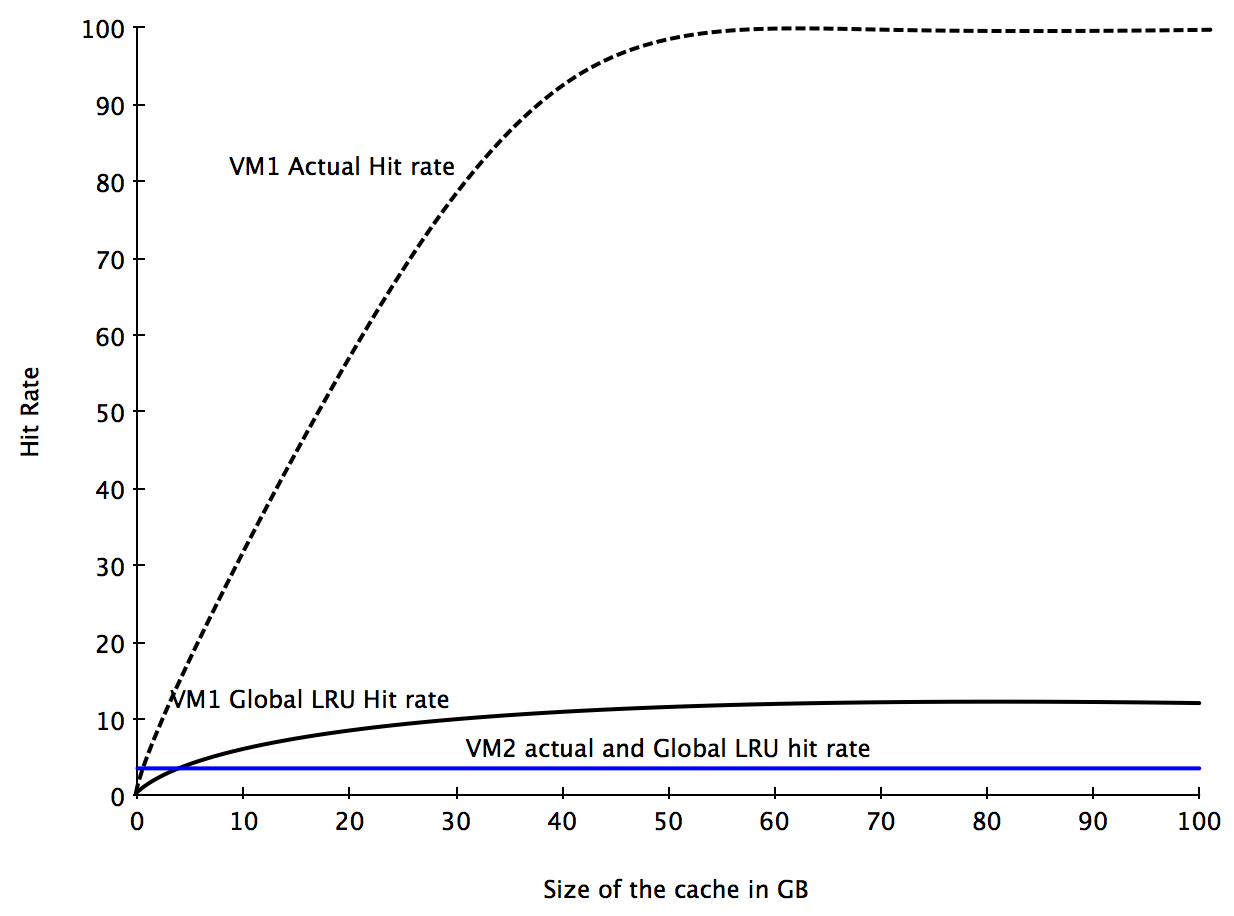
\includegraphics[width=3in]{figures/hitrate_fake}
\caption{VMs competing for resources}
\label{fig:compete}
\end{figure}

The need for partitioning the SSD cache has been studied in [vCacheShare, ...]. To illustrate we conduct a simple experiment where two VMs, namely VM1 and VM2, residing in the same host share a caching device. From figure XX, one can see that VM1 has a high random I/O with a very low hit ratio while VM2 has a low I/O but has a high hit rate. Figure~\ref{fig:compete} , shows that despite VM2 could benefit largely from a cache, it has a very low space allocation in the cache, due to contention from VM1. From figure XX and YY, one can infer that contention can make a cache entirely unusable.

\note{Insert a table of various SSD costs}


\subsection{The case for two-layer cache}

As we can see from the figure, there are a number of devices that can be adopted to use as a cache. However the widespread adoption of these devices have always remained slow, mainly because of the difficulty to determine the combination of devices the will give the maximum performance with minimal cost. Another major pain point to utilize these devices efficiently; a bad partitioning strategy would degrade the performance otherwise. The optimization is complex due to the wide variety of devices as well as the workloads in the datacenter.

To overcome these challenges, we propose a dynamically scaling algorithm that not only seemlessly scales to multi-tier caches, but also optimize the caching space for both maximum utilization and overall hit rate of the system. Quantifying the performance gains from the selection of the devices is quite challenging. To this end we propose a cache utility model that quantifies and allows us to maximize the cache utilization and hit rate.

Each VM in a data center come with their own priority and Service Level Agreement. The priority if not explicitly mentioned, it can be inferred from the type of service they request at the time of their creation. VMs that run web services expect to have a very minimal latency as the response time is the most important criterion. On the other hand, VMs that run database servers, don't care about latency as much, but they want to optimize for throughput. It is the same with batch jobs, where the life time of the jobs is very short- jobs come in for a quick computation, and once they are done, there is a single reply with the result and they are done.

Optimizing for each of the different kinds of VMs on a single physical machine is a very diffucult task. Instead, we take the latency as a common denominator and use it as a tuning parameter to meet the SLAs of the VMs. For instance, interactive VMs that has a very low I/O, but a very high hit rate can be ``separated" and placed in the lowest latency cache for high reponsiveness. 

The future that we envision with our system is that, a system administrator should be able to insert one or more flash devices into a host running our architecture and should be able to get instant benefit from it. Scalability is the key.

\section{Overview}

\subsection{Hit Ratio Curves}

Hit ratio curves as a function of cache size gives us an estimate of the percentage of cache hits for any given cache size. A common method to calculate the HRC is by calculating the \emph{Reuse Distance} for every block request. A Reuse Distance (RD) is the number of unique blocks between two consecutive accesses of a given block.

RD calculation for every block for a workload is computationally intensive. All the block requests for a given workload needs to be saved in the memory, and for every block request, the previous occurrence of that request has to be found and the number of unique elements between the two occurrences needs to be calculated. A naive implementation of Mattson's algorithm thus takes $\mathcal{O}(n\log{}n)$ space, where $n$ is the size of the trace, and $\mathcal{O}(n\log{}nm)$ runtime where $m$ is the number of unique blocks in the trace.

Recently there have been some works [Parda, Shards, CounterStack] that calculate RD in sublinear time with constant space. CounterStack algorithm uses a counter for each of the block request, that holds the counter for the number of blocks requested after the counter for a particular block has been initialized. Comparing the counter of a block with other blocks give the RD of that block. The space is exponentially reduced by the usage of Hyperloglog [ref] data structure for each of the counters and by various other techniques such as downsampling.

Shards on the other hand uses hashing to calculate the hash value of the block address and modulo the value by a user defined constant. If the resulting value is lesser than another user defined threshold, the block address is retained for calculating RD, if not, the block address is discarded. The authors of Shards claim that by just using the very minimal sample of uniformly distrubuted block addresses, they are able to calculate the RD values with very little error.

In our work, we chose to use a variation of Mattson's Algorithm instead of adopting Shards or CounterStack for two simple reasons- First, our algorithm has a very small time window within which we calculate the RD of the blocks that have been requested. This means that our sample is already very small, in the order of tens of Kilobytes. Using Shards or CounterStack on such a small sample size is highly inefficient and leads to inaccuracies, as these methods work well with a larger sample size. Second, we were aiming to avoid serious computationally intesive calculations for calculating RD, as we would have to do this several hundreds or thousands of times depending on our time window.

 Our variation of Mattson algorithm is shown in listingX. We maintain a global counter to count the number of block requests, and a hastable that stores the block adresses as the key and an array of indexes as it's values. This array will store the counter(s) at which the given block(key) was requested. For every block request, we look up our hashtable if the block address exists. If it does, we append the current counter value to the block address, else we insert the block address into the hastable with it's initial value as the counter's current value.

 If we want to calculate the reuse distance, usually at the end of a timewindow, the hastable is iterated one key at a time and the pairwise-difference between each of the values of the keys gives us the approximate reuse distance. A cdf of all the pairwise-distances gives us an approximate HRC as a function of the reuse distance. \note{Need better explanation}

 \subsection{Reuse Intensity}

\emph{Reuse Intesity} is used as a measure to capture sudden bursts in hit ratio, as opposed to RD which is used to capture the overall trend of the hit ratio for a given time window. For certain web services, such as stock market providers, capturing quick bursts in trend is vital. To this end, $$ RI = \frac{unique blocks}{total blocks} $$ captures the sudden bursts in Hit Ratio. We calculate this value once every second. The overhead incurred by this calculation is very minimal compared to the other computations in our algorithm. So, calcualting this value in the background/parallely to other computations results in zero overhead. \note{is this statement true?}

\subsection{Cache Utility model}

\note{See github discussion}

We run the optimazation algorithm in two parts/stages. Our solver uses simnulated Annealing algorithm. We split the hit ratio curve into two parts. The division point is the size of the FC. We find the optimal cache space for the VMs for FC. Once we solve for FC, we then solve the ``remaining" i.e. from size(FC) + 1 to size(SC + FC) as shown in figureX.

\section{Evaluation}

\subsection{Experimental Setup}
\subsection{Workload Analysis}
\subsection{Performance Metrics}
\subsection{Experiments}

\section{Related Work}

The most closest work to ours, from which we extended our work upon is by Meng et. al.~\cite{meng_vcacheshare:_2014}

\section{Conclusion}


% \bibliographystyle{abbrv}
% \bibliography{citations}

% that's all folks
\end{document}
